\chapter{Теоретические основы}
\label{cha:theory}

\section{Основные понятия теории графов}

Теория графов изучает графы — абстрактные структуры, состоящие из вершин (узлов) и рёбер (связей между узлами). Основные понятия теории графов включают следующие элементы:

Граф \(G = (V, E)\) состоит из множества вершин \(V\) и множества рёбер \(E\), где каждое ребро представляет собой пару вершин. Граф может быть ориентированным (если рёбра имеют направление) и неориентированным (если рёбра не имеют направления).

Матрица смежности \(A\) графа \(G\) размером \(n \times n\) (где \(|V|\) обозначает количество вершин графа и равно \(n\), задается как квадратная матрица, в которой элемент \(a_{ij}\) равен 1, если существует ребро между вершинами \(v_i\) и \(v_j\), в противном случае 0. Для ориентированного графа матрица смежности не обязательно симметрична\cite{7}.

Степень вершины \(v\) в графе \(G\) (обозначаемая как \(\deg(v)\)) - это количество рёбер, связанных с данной вершиной. В ориентированном графе различают входящую степень (\(\deg_{in}(v)\)) и исходящую степень (\(\deg_{out}(v)\))\cite{6}.

Граф \(G\) называется связным, если существует путь между любой парой вершин. Для ориентированных графов используется понятие сильной связности, когда для любой пары вершин \(u\) и \(v\) существует ориентированный путь как от \(u\) к \(v\), так и от \(v\) к \(u\)\cite{8}.

\section{Связь между случайными блужданиями и электрическими сопротивлениями}

Случайное блуждание на графе \(G\) представляет собой процесс, при котором на каждом шаге изменяется состояние случайного процесса, заключающееся в перемещении из текущей вершины в одну из соседних вершин, выбранную независимым образом с равной вероятностью. Этот процесс можно моделировать с помощью матрицы переходов \(P\), где элемент \(p_{ij}\) представляет собой вероятность перехода из вершины \(v_i\) в вершину \(v_j\).

Электрические сети могут быть представлены в виде графов, где вершины соответствуют узлам сети, а рёбра - проводникам или линиям связи. Для анализа таких сетей используется подход основаный на теории графов и модели случайных блужданий.

Сопротивление между двумя узлами \(i\) и \(j\) в электрической сети можно вычислить, моделируя сеть в виде графа и используя случайные блуждания. В частности, среднее время первого попадания из узла \(i\) в узел \(j\) и обратно (commute time) тесно связано с электрическим сопротивлением между этими узлами.

Для расчета среднего времени первого попадания (hitting time) можно использовать следующую формулу. Пусть \(G\) - граф, где \(V\) - множество вершин, \(E\) - множество рёбер. Например, рассмотрим однородное случайное блуждание, при котором вероятность перехода из одной вершины в любую соседнюю вершину одинакова и равна \(1/d(j)\). А среднее время случайного перемещения из \(i\) в \(j\) и обратно будет тогда  равно \(1/d(j) + 1/d(i)\), где \(d(x)\) - степень вершины \(x\). 

\section{Время первого попадания}
\begin{theorem}[Время первого попадания]

Среднее время первого попадания в вершину \(j\) из вершины \(i\) определяется как разность потенциалов (Сценарий A):

$$\phi_{ij} = H_{ij}  \eqno(1)$$

\begin{figure}[h]
    \centering
    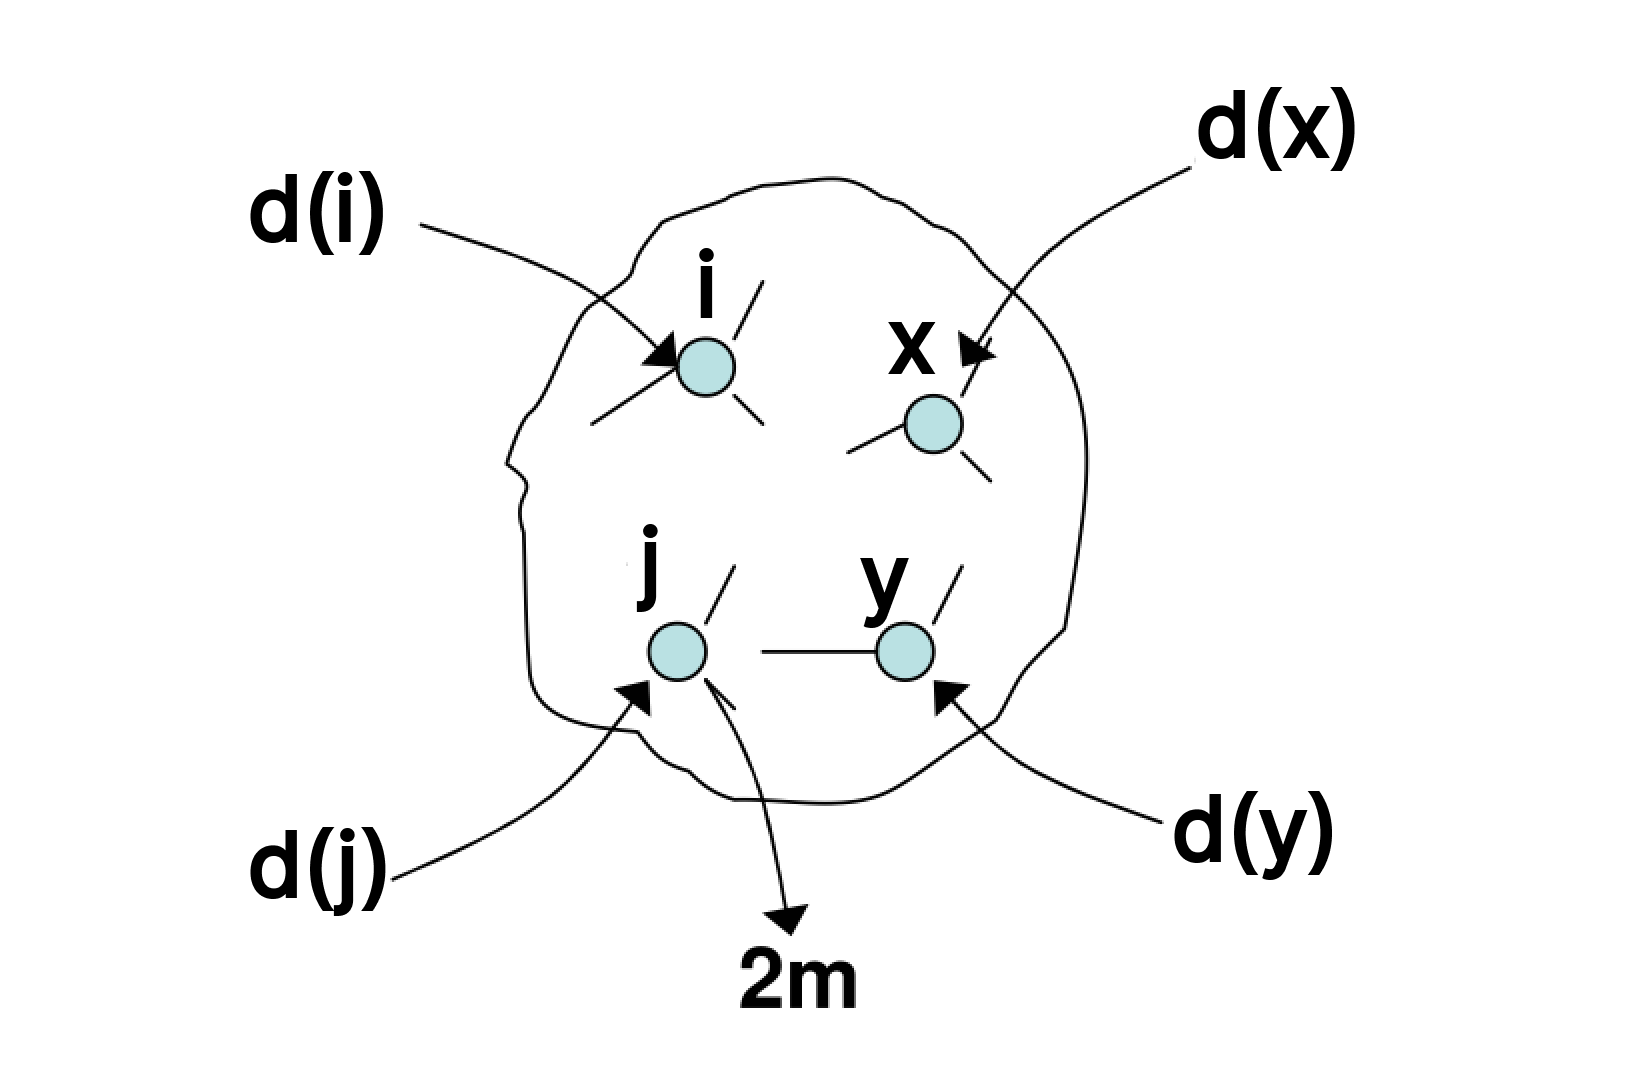
\includegraphics[width=0.3\linewidth]{figures/A.png}
    \caption{Сценарий A}
\end{figure}
\end{theorem}

Теорема взята из \cite{1}.

\begin{proof}

Для доказательства данной теоремы введем законы Кирхгофа и Ома:

\begin{itemize}
    \item Суммарный ток в вершине и из нее равен нулю (K1) \cite{4}
    \item Сумма разностей потенциалов в любом цикле равна нулю (K2) \cite{4}
    \item Ток, протекающий по любому ребру, равен \(\text{разности потенциалов} \text{ деленная на } \text{сопротивление}\) (Закон Ома) \cite{5}
\end{itemize}


Теперь рассмотрим любую вершину \(i \in V\). Используя законы Кирхгофа и Ома, мы имеем:

$$d(i) = \sum_{(i, x) \in E} \text{текущая } i \to x  \text{(K1)} $$
$$= \sum_{(i, x) \in E} \phi_{ix}   \text{(Закон Ома)} $$
$$= \sum_{(i, x) \in E} (\phi_{ij} - \phi_{xj}) \text{(K2)} $$
$$= d(i)\phi_{ij} - \sum_{(i, x) \in E} \phi_{xj} $$

Преобразование даст:

$$
\phi_{ij} = 
\begin{cases} 
0 &  i = j \\
1 + \frac{1}{d(i)} \sum\limits_{(i,x) \in E} \phi_{xj} &  i \neq j
\end{cases} 
\eqno(2)
$$


С другой стороны, рассмотрим случайное блуждание, начинающееся с \(i\). Рассматривая только первый шаг этой прогулки, мы видим, что время попадания \(H_{ij}\) удовлетворяет следующим условиям:

$$
H_{ij} = 
\begin{cases} 
0 &  i = j \\
1 + \frac{1}{d(i)} \sum\limits_{(i,x) \in E} H_{xj} &  i \neq j
\end{cases} 
\eqno(3)
$$

Но это точно такая же система линейных уравнений, как и (2), удовлетворяемая \(\phi_{ij}\). Поскольку мы знаем, что эта система имеет единственное решение (потенциалы однозначно определяются потоками тока), мы выводим, что:

$$H_{ij} =  \phi_{ij}  \forall i \in V  $$

\end{proof}

\section{Эффективное сопротивление}

Эффективное сопротивление (резистивное расстояние) \(\Omega_{vw}(\mathcal{L})\) между вершинами \(u\) и \(v\) в графе с равным сопротивлением \(r\) на всех рёбрах определяется как сумма взвешенных квадратов разностей между компонентами собственных векторов графа для всех пар узлов \(v\) и \(w\). В частности, для каждого узла \(v\) и \(w\) вычисляется разность компонент собственных векторов \(\psi_{jv}\) и \(\psi_{jw}\), которые соответствуют ненулевым собственным значениям \(\lambda_j(\mathcal{L})\) лапласиана. Затем, каждая разность возводится в квадрат, делится на соответствующее собственное значение, и все такие дроби суммируются для всех j от 2 до n. :

$$ \Omega_{vw}(\mathcal{L}) = \sum_{j=2}^{n} \frac{1}{\lambda_j(\mathcal{L})} (\psi_{jv} - \psi_{jw})^2 \eqno(4.1)$$


Данная запись присутствует в \cite{2} на стр. 11, но для  удобства, формула (4.1) будет видоизменена:


$$ R_{ij} = \sum_{k=1}^{n-1} \frac{(u_{ki} - u_{kj})^2}{\lambda_k} \eqno(4.2)$$


В формуле 4.2 \(\lambda_k\) – это собственные значения Лапласиана, где \(\lambda_0 = 0\), \(u_{ki}\) и \(u_{kj}\) - i-я и j-я компоненты k-го собственного вектора Лапласиана, а n – это вершины. Лапласиан, или матрица Лапласа определяется как матрица степеней \(D\) минус матрица смежности \(A\):
$$  \mathcal{L} = D - A  $$


\section{Время возвращения}
\begin{theorem}[Время возвращения]
Среднее время случайного перемещения из i в j и обратно определяется как cреднее время первого попадания в вершину \(j\) из вершины \(i\) плюс cреднее время первого попадания в вершину \(i\) из вершины \(j\) иле же как количество ребер \(m\) умноженное на эффективное сопротивление \(R_{ij}\) умноженное на два.

$$ C_{ij} = H_{ij} + H_{ji} = 2mR_{ij}\eqno(5)$$
\end{theorem}

Формула взята из \cite{3}, стр. 577.

\begin{proof}

Для доказательства используем сценарий B, который похож на сценарий A, за исключением того, что мы удаляем \(2m\) единицы тока с узла \(i\), а не с узла \(j\). Обозначая разность потенциалов в сценарии B через \(\phi^{'}\), мы имеем, согласно теореме 1:
$$\phi_{ji}^{'} = H_{ji} \eqno(6)$$

Теперь рассмотрим сценарий C, который похож на сценарий B, но с обратными токами. Обозначив разность потенциалов в этом сценарии через \(\phi''\), мы получаем:

$$\phi_{ij}^{''} = \phi_{ji}^{'} = H_{ji} \eqno(7)$$

\begin{figure}[h]
    \centering
    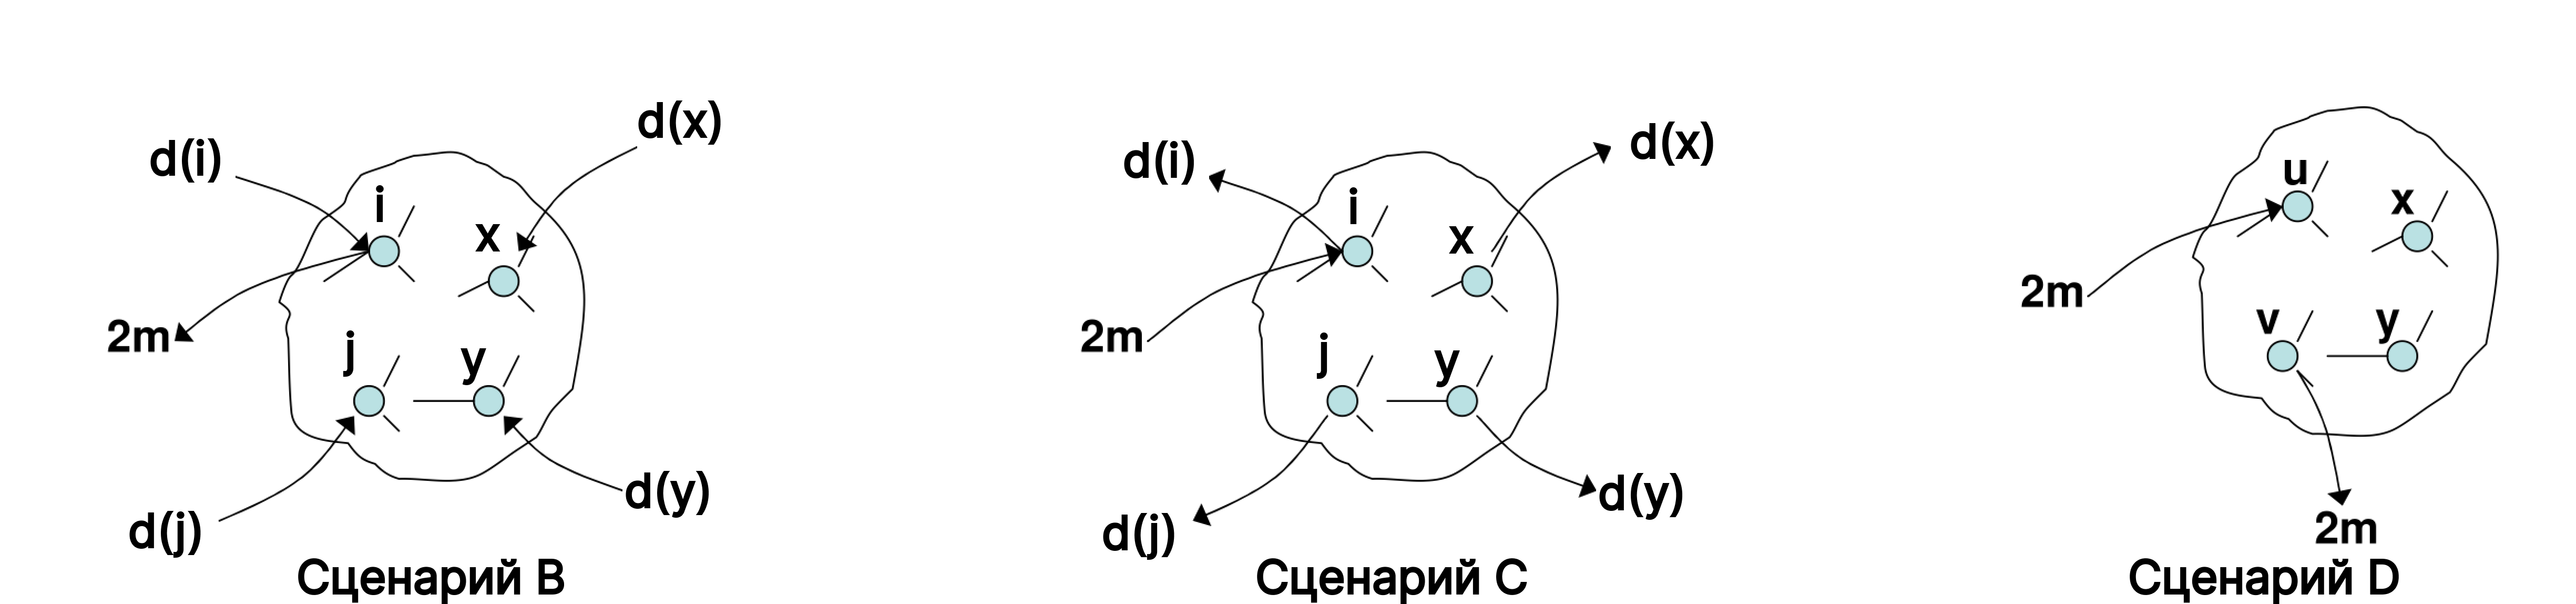
\includegraphics[width=1\linewidth]{figures/BCD.png}
    \caption{Сценарий B,C и D}
\end{figure}

Наконец, рассмотрим сценарий D, который представляет собой сумму сценариев A и C. В силу линейности и обозначения потенциальные различия в сценарии D через \(\phi^{'''}\), мы имеем:

$$\phi_{ij}^{'''} = \phi_{ij} + \phi_{ij}^{''}= H_{ij} = H_{ji} \eqno(8)$$

Так как \(\phi_{ij}^{''}\) – это разность потенциалов, необходимая для перемещения \(2m\) единиц тока из \(i\) в \(j\), поэтому по закону Ома она равна \(2mR_{ij}\).
\end{proof}
